\documentclass{beamer}
\let\vec\mathbf
\mode<presentation>
\usepackage{amsmath}
\usepackage{amssymb}
%\usepackage{advdate}
\usepackage{adjustbox}
%\usepackage{subcaption}
\usepackage{enumitem}
\usepackage{multicol}
\usepackage{mathtools}
\usepackage{listings}
\usepackage{url}
\usetheme{Boadilla}
\usecolortheme{lily}
\setbeamertemplate{footline}
{
  \leavevmode%
  \hbox{%
  \begin{beamercolorbox}[wd=\paperwidth,ht=2.25ex,dp=1ex,right]{author in head/foot}%
    \insertframenumber{} / \inserttotalframenumber\hspace*{2ex} 
  \end{beamercolorbox}}%
  \vskip0pt%
}
\setbeamertemplate{navigation symbols}{}
\providecommand{\nCr}[2]{\,^{#1}C_{#2}} % nCr
\providecommand{\nPr}[2]{\,^{#1}P_{#2}} % nPr
\providecommand{\mbf}{\mathbf}
\providecommand{\pr}[1]{\ensuremath{\Pr\left(#1\right)}}
\providecommand{\qfunc}[1]{\ensuremath{Q\left(#1\right)}}
\providecommand{\sbrak}[1]{\ensuremath{{}\left[#1\right]}}
\providecommand{\lsbrak}[1]{\ensuremath{{}\left[#1\right.}}
\providecommand{\rsbrak}[1]{\ensuremath{{}\left.#1\right]}}
\providecommand{\brak}[1]{\ensuremath{\left(#1\right)}}
\providecommand{\lbrak}[1]{\ensuremath{\left(#1\right.}}
\providecommand{\rbrak}[1]{\ensuremath{\left.#1\right)}}
\providecommand{\cbrak}[1]{\ensuremath{\left\{#1\right\}}}
\providecommand{\lcbrak}[1]{\ensuremath{\left\{#1\right.}}
\providecommand{\rcbrak}[1]{\ensuremath{\left.#1\right\}}}
\theoremstyle{remark}
\newtheorem{rem}{Remark}
\newcommand{\sgn}{\mathop{\mathrm{sgn}}}

\providecommand{\res}[1]{\Res\displaylimits_{#1}} 
\providecommand{\norm}[1]{\left\lVert#1\right\rVert}
\providecommand{\mtx}[1]{\mathbf{#1}}

\providecommand{\fourier}{\overset{\mathcal{F}}{ \rightleftharpoons}}
%\providecommand{\hilbert}{\overset{\mathcal{H}}{ \rightleftharpoons}}
\providecommand{\system}{\overset{\mathcal{H}}{ \longleftrightarrow}}
	%\newcommand{\solution}[2]{\textbf{Solution:}{#1}}
%\newcommand{\solution}{\noindent \textbf{Solution: }}align
\providecommand{\dec}[2]{\ensuremath{\overset{#1}{\underset{#2}{\gtrless}}}}
\newcommand{\myvec}[1]{\ensuremath{\begin{pmatrix}#1\end{pmatrix}}}

\title{Matrices in Geometry - 2.4.7}
\author{EE25BTECH11017 Mahesh Chollangi}
\date{Sept, 2025}

\begin{document}

\maketitle

\frame{\titlepage}
\begin{frame}{Question}
    Find the projection of the vector $\vec{a} = 2\hat{i}+3\hat{j}+2\hat{k}$ on the vector $\vec{b} = \hat{i}+2\hat{j}+\hat{k}$.\\
\end{frame}

\begin{frame}{Given Information}
    Let the vectors be represented as \textbf{A}, \textbf{B} respectively. Given by

\begin{align}
    \textbf{A} = \myvec{2 \\ 3 \\ 2}, \textbf{B} = \myvec{1 \\ 2\\ 1} 
    \label{0.1}
\end{align}
\end{frame}

\begin{frame}{Solution}
    Mathematically, the projection of the vector \textbf{A} on the vector \textbf{B} is given by some vector \textbf{D},

\begin{align}
    \textbf{D} = k\textbf{B}\text{, such that } (\textbf{A}-\textbf{D})^\text{T}\textbf{D}=0
    \label{0.2}
\end{align}
\end{frame}

\begin{frame}{Continuation}
    yielding,

\begin{align}
    (\textbf{A}-k\textbf{B})^\text{T}\textbf{B}=0
    \label{0.3}
\end{align}

or,


\begin{align}
    k=\frac{\textbf{A}^\text{T}\textbf{B}}{\norm{\textbf{B}}^2} \implies \textbf{D} = \frac{\textbf{A}^\text{T}\textbf{B}}{\norm{\textbf{B}}^2}\textbf{B}
    \label{0.4}
\end{align}
\end{frame}

\begin{frame}{Continuation}
    On substituting the values,

\begin{align}
    \textbf{D} = \frac{\brak{\myvec{2\\3\\2}}^\text{T}\myvec{1\\2\\1}}{\norm{\myvec{1\\2\\1}}^2}\myvec{1\\2\\1}
    \label{0.5}
\end{align}
\end{frame}

\begin{frame}{Final Answer}
    On calculation, this gives us,

\begin{align}
    \textbf{D} = \myvec{5/3\\10/3\\5/3}
    \label{0.6}
\end{align}
\end{frame}

\begin{frame}[fragile]
\frametitle{C code}
\begin{lstlisting}

#include <stdio.h>

void vector_projection(double a[3], double b[3],
double proj[3]) {
double b_norm_sq = b[0]*b[0] + b[1]*b[1] + b[2]*b[2];
double dot_product = a[0]*b[0] + a[1]*b[1] + a[2]*b[2];

    double scalar = dot_product / b_norm_sq;

    proj[0] = scalar * b[0];
    proj[1] = scalar * b[1];
    proj[2] = scalar * b[2];
}


\end{lstlisting}
\end{frame}

\begin{frame}[fragile]
\frametitle{Python code}
\begin{lstlisting}

import numpy as np
import matplotlib.pyplot as plt
from mpl_toolkits.mplot3d import Axes3D

# Define vectors
a = np.array([2, 3, 2])
b = np.array([1, 2, 1])

# Calculate projection of a on b
b_norm = b / np.linalg.norm(b)
proj_a_on_b = np.dot(a, b_norm) * b_norm

# Plotting
fig = plt.figure()
ax = fig.add_subplot(111, projection='3d')


\end{lstlisting}
\end{frame}


\begin{frame}[fragile]
\frametitle{Python code}
\begin{lstlisting}

# Plot vector a
ax.quiver(0, 0, 0, a[0], a[1], a[2], color='r', 
label='Vector a')

# Plot vector b
ax.quiver(0, 0, 0, b[0], b[1], b[2], color='b', 
label='Vector b')

# Plot projection of a on b
ax.quiver(0, 0, 0,proj_a_on_b[0],proj_a_on_b[1],
proj_a_on_b[2],color='g',label='Projection of a on b')

# Setting the plot limits
max_val = max(np.linalg.norm(a),np.linalg.norm(b))+1
ax.set_xlim([0, max_val])
ax.set_ylim([0, max_val])

\end{lstlisting}
\end{frame}

\begin{frame}[fragile]
\frametitle{Python code}
\begin{lstlisting}

ax.set_zlim([0, max_val])
ax.set_xlabel('X axis')
ax.set_ylabel('Y axis')
ax.set_zlabel('Z axis')
ax.legend()
plt.title('Vector Projection: a on b')
plt.show()

\end{lstlisting}
\end{frame}


\begin{frame}{Plot}
    \begin{figure}[H]
    \centering
    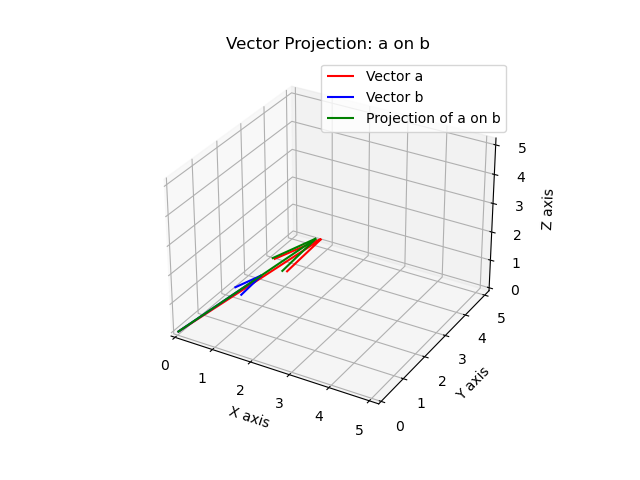
\includegraphics[width=0.8\columnwidth]{Figs/Figure_2.png}
    \caption{3D Plot}
    \label{3D Plot}
\end{figure}
\end{frame}
\end{document}